\label{2}
\part{Controles}
\section{Movimentos à disposição}

Dentro do jogo o usuário terá movimentos obtidos quanto do teclado e quanto do mouse que servem para jogabilidade e navegar entre as telas do jogo.

\subsection{Teclado}

O jogador terá a sua disposição o usos das teclas 'r' para reiniciar o jogo, a tecla 'c' para continuar em determinadas telas e mais as teclas da imagem abaixo.

\label{teclas}
\begin{figure}[h]
	\centering
	\caption{Imagem ilustrativa das rela\c{c}\~oes das teclas com o carro}
		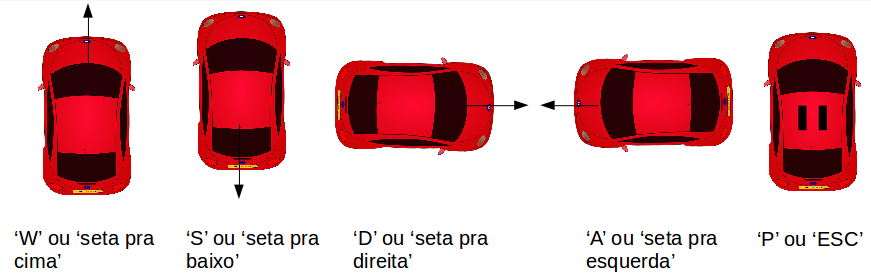
\includegraphics[keepaspectratio=true,scale=0.5]{figuras/movimentos}
\end{figure}

\subsection{Mouse}

O mouse será o meio usado para a movimentação da câmera de jogo.
